% Anexo IV — Planimetría de recolección, impulsión y tratamiento. Origen: v3.0, Anexo D.
\chapter{Planimetría de recolección, impulsión y tratamiento}
\label{anx:planimetria-hidraulica}

Las \cref{fig:lamina-2-1a,fig:lamina-2-1b,fig:lamina-2-2a,fig:lamina-2-2b,fig:lamina-2-3,fig:lamina-2-4} presentan las láminas del sistema hidráulico y de tratamiento.

\begin{figure}[p]
  \centering
  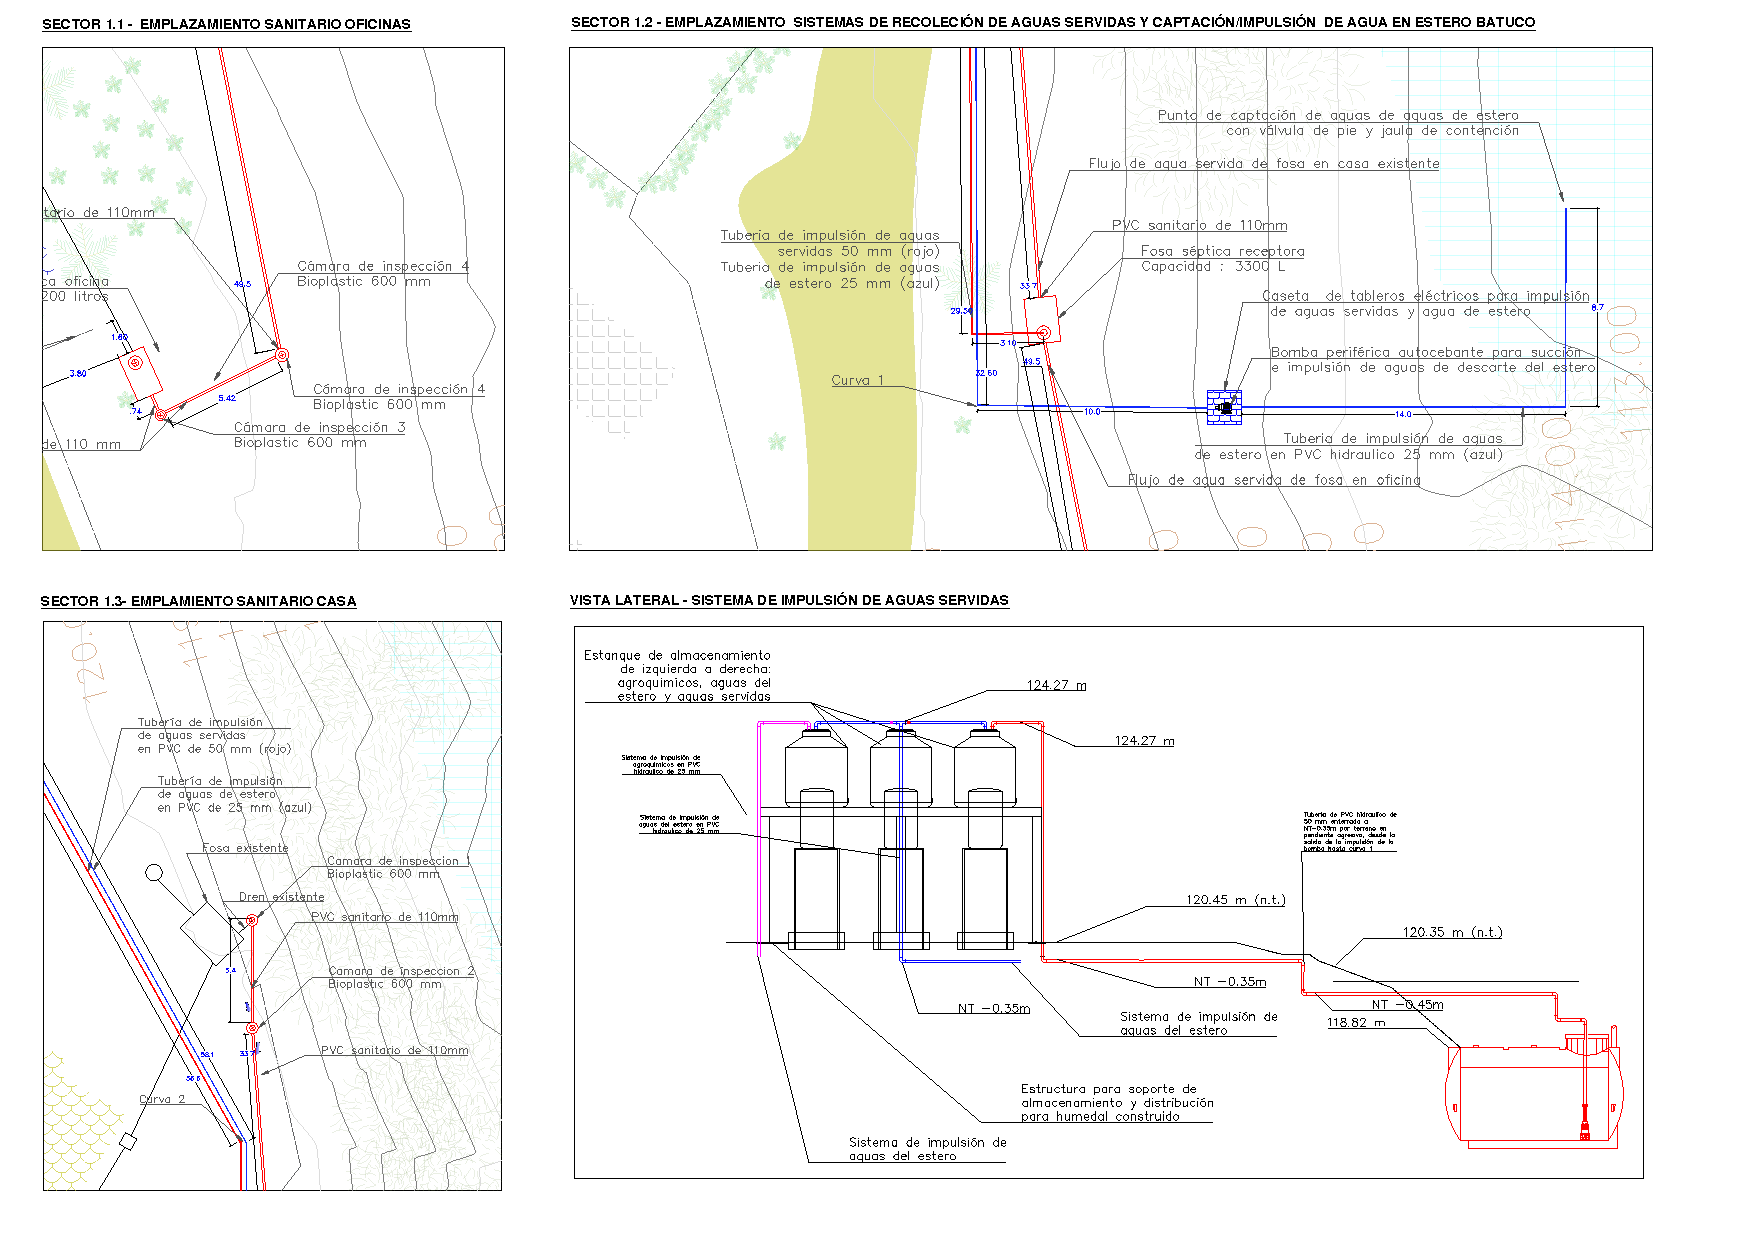
\includegraphics[angle=90, height=0.82\textheight, width=\textwidth, keepaspectratio]{planos/2_1_recoleccion-impulsion-planta.pdf}
  \caption{Lámina 2.1: planta del sistema de recolección e impulsión. Fuente: elaboración propia.}
  \label{fig:lamina-2-1a}
\end{figure}

\begin{figure}[p]
  \centering
  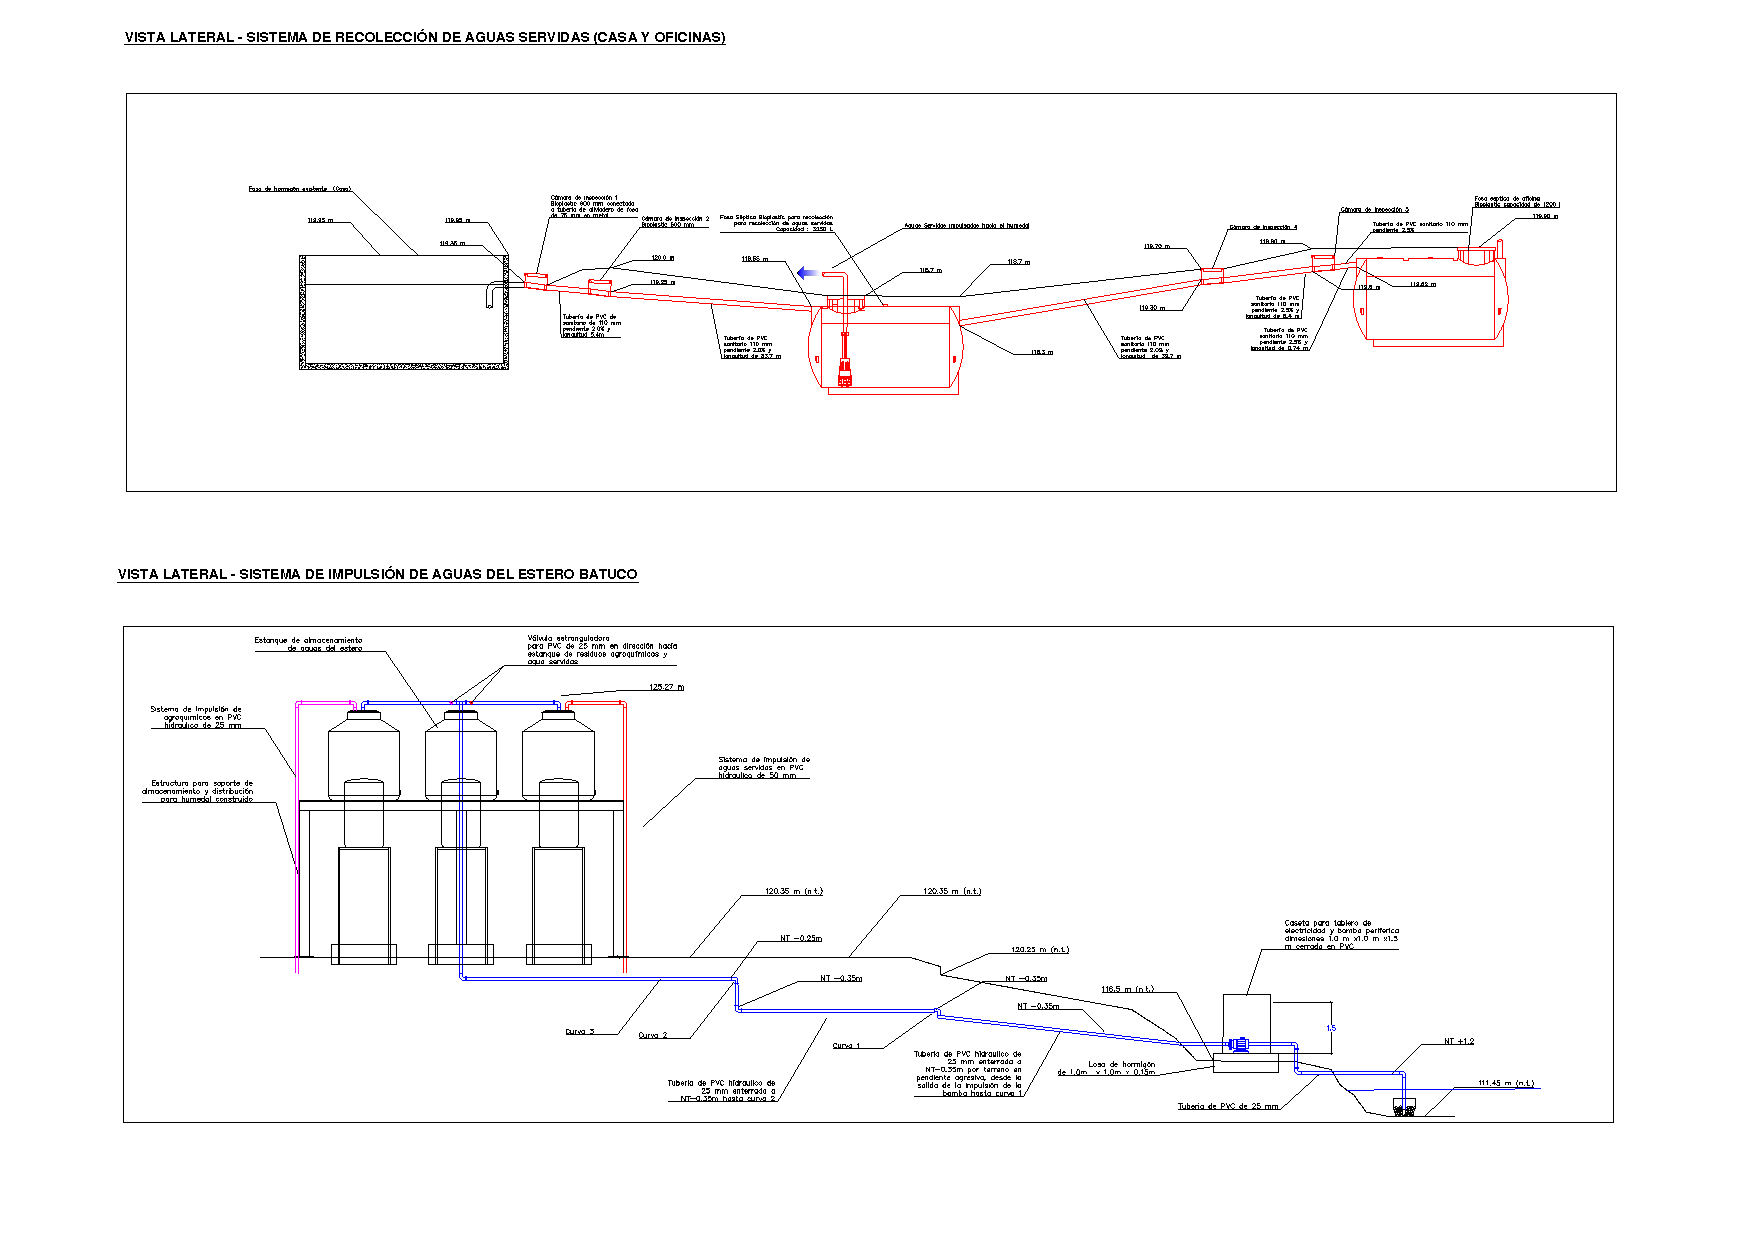
\includegraphics[angle=90, height=0.82\textheight, width=\textwidth, keepaspectratio]{planos/2_1_recoleccion-impulsion-vistas-laterales.pdf}
  \caption{Lámina 2.1: vistas laterales del sistema de recolección e impulsión. Fuente: elaboración propia.}
  \label{fig:lamina-2-1b}
\end{figure}

\begin{figure}[p]
  \centering
  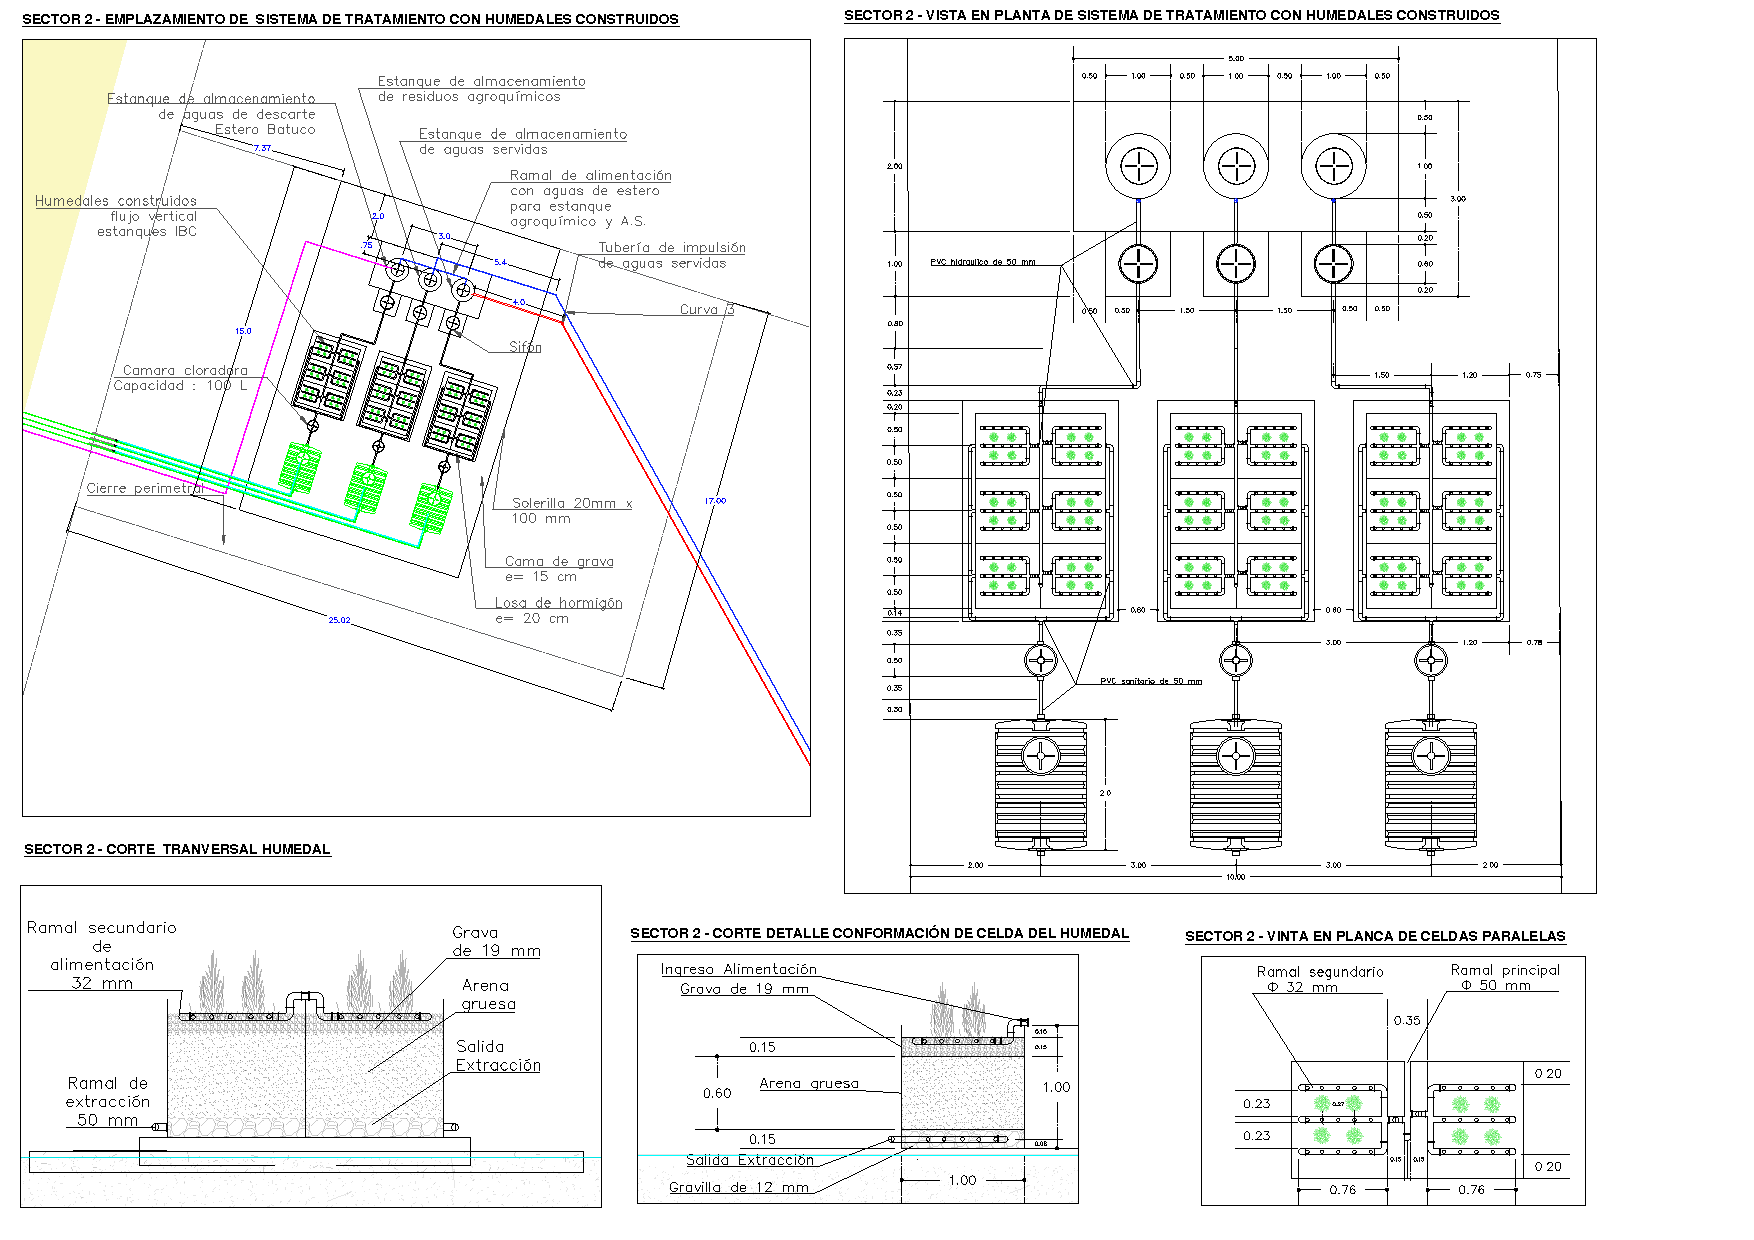
\includegraphics[angle=90, height=0.82\textheight, width=\textwidth, keepaspectratio]{planos/2_2_humedales-planta.pdf}
  \caption{Lámina 2.2: planta general de los humedales construidos. Fuente: elaboración propia.}
  \label{fig:lamina-2-2a}
\end{figure}

\begin{figure}[p]
  \centering
  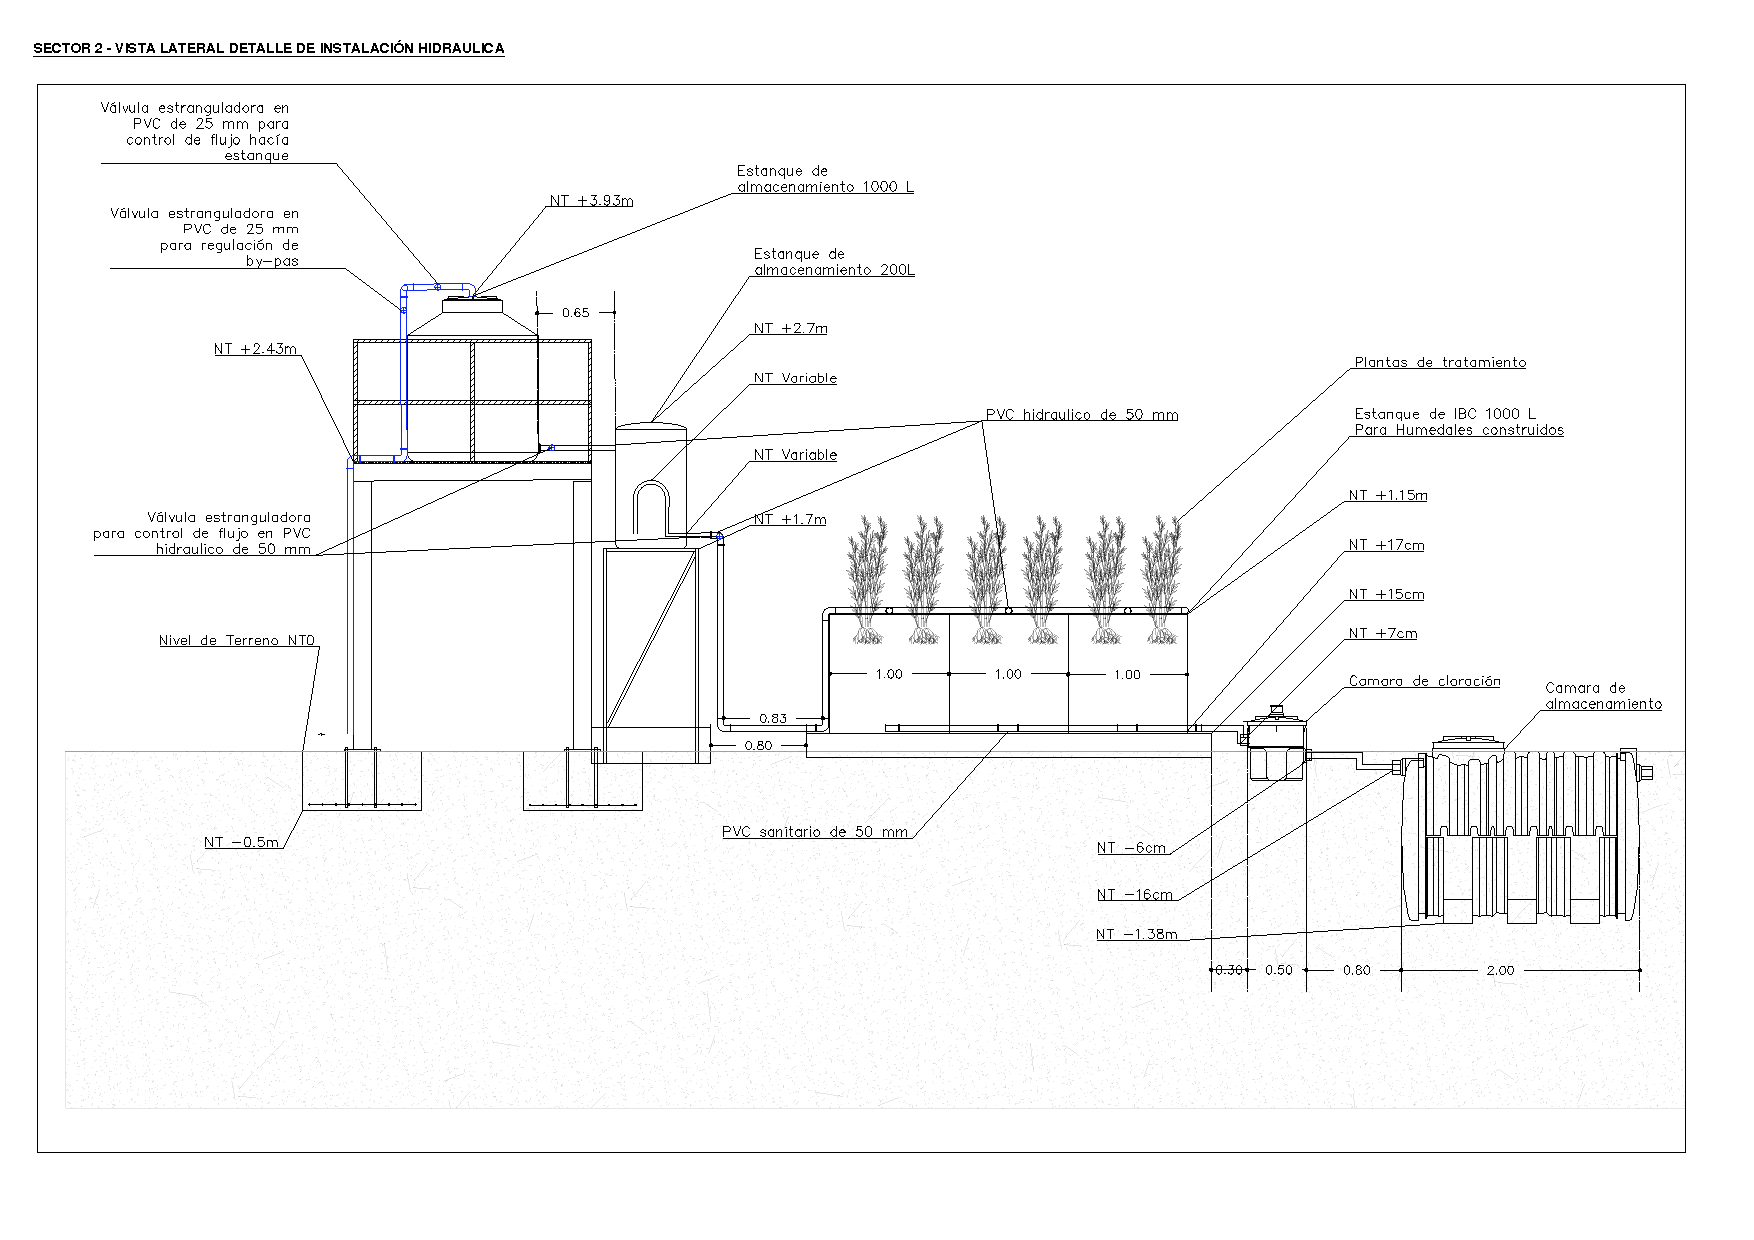
\includegraphics[angle=90, height=0.82\textheight, width=\textwidth, keepaspectratio]{planos/2_2_humedales-vista-lateral.pdf}
  \caption{Lámina 2.2: vista lateral y corte de los humedales construidos. Fuente: elaboración propia.}
  \label{fig:lamina-2-2b}
\end{figure}

\begin{figure}[p]
  \centering
  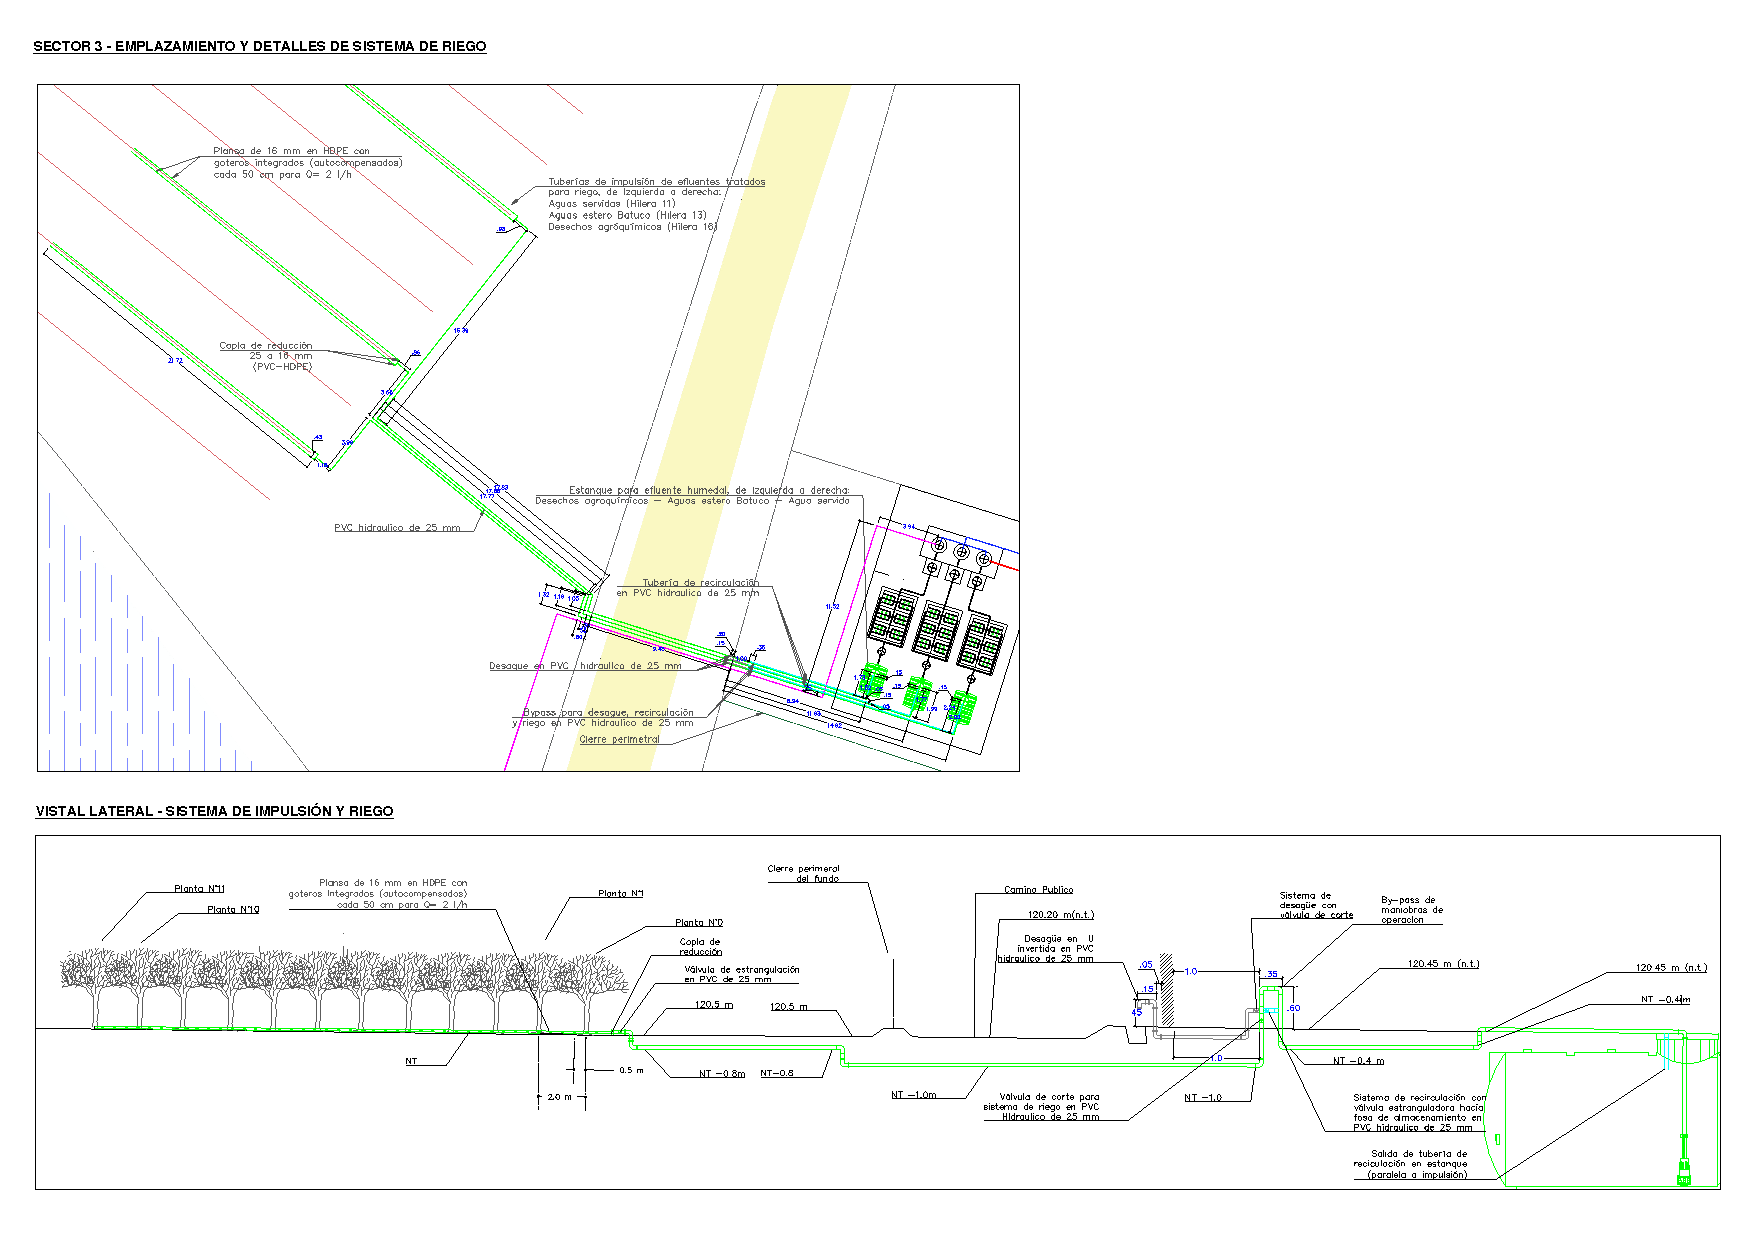
\includegraphics[angle=90, height=0.82\textheight, width=\textwidth, keepaspectratio]{planos/2_3_riego-impulsion.pdf}
  \caption{Lámina 2.3: sistema de riego e impulsión. Fuente: elaboración propia.}
  \label{fig:lamina-2-3}
\end{figure}

\begin{figure}[p]
  \centering
  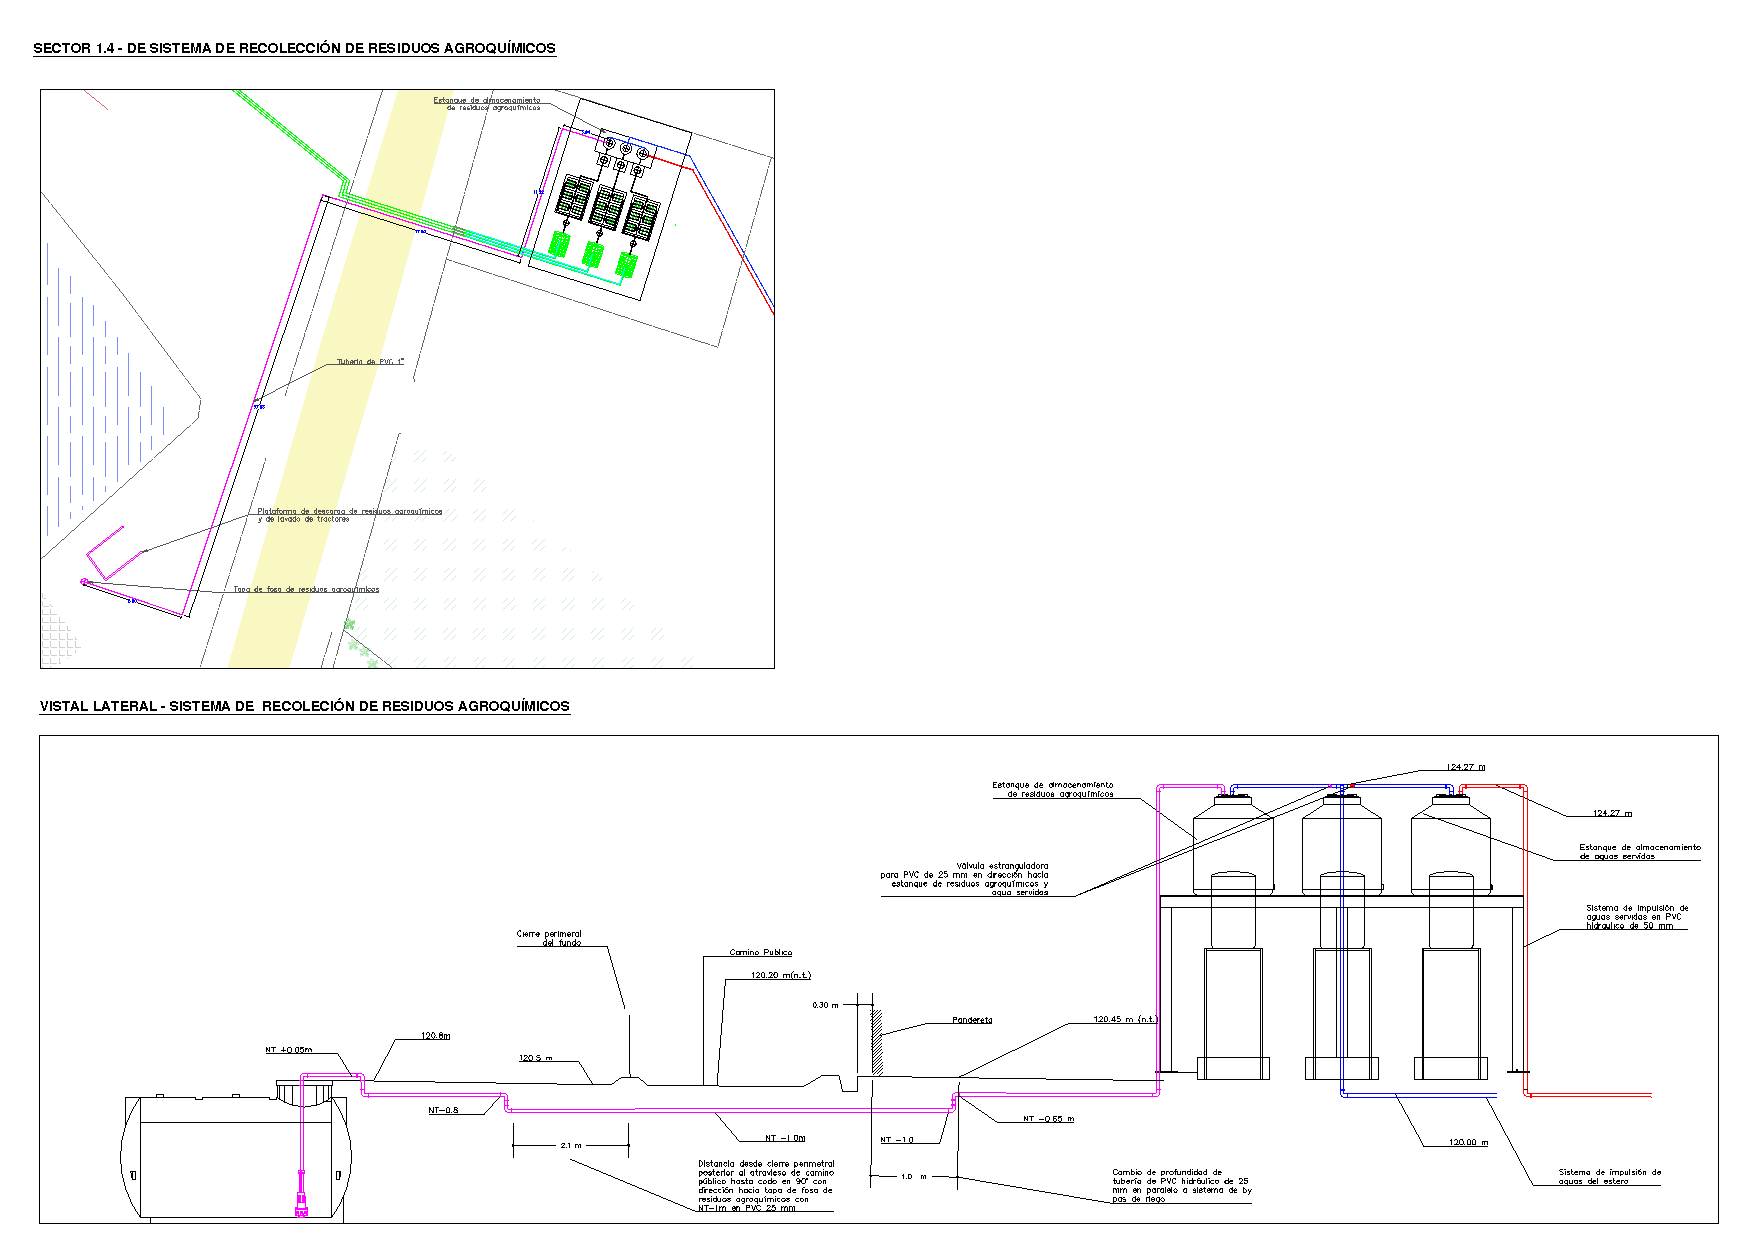
\includegraphics[angle=90, height=0.82\textheight, width=\textwidth, keepaspectratio]{planos/2_4_recoleccion-agroquimicos.pdf}
  \caption{Lámina 2.4: sistema de recolección de residuos agroquímicos. Fuente: elaboración propia.}
  \label{fig:lamina-2-4}
\end{figure}

